%%%%%%%%%%%%%%%%%%%%%%%%%%%%%%%%%%%%%%%%%%%%%%%%%%%%%%%%%%%%%%%%%%%%%%%%%%%
%%
%%  ch-atmshowers.tex
%%
%%  Created: Fri Oct 10 14:24:37 1997
%%  Author.: Jose Carlos Gonzalez
%%  Notes..:
%%          
%%-------------------------------------------------------------------------
%% Filename: $RCSfile$
%% Revision: $Revision$
%% Date:     $Date$
%%%%%%%%%%%%%%%%%%%%%%%%%%%%%%%%%%%%%%%%%%%%%%%%%%%%%%%%%%%%%%%%%%%%%%%%%%%


\chapter{Atmospheric gamma and cosmic-ray showers}
\label{chapter:atmshowers}

The particles that conform the CRAD, when entering into the Earth's
atmosphere, interact with molecules and atoms, producing secondary
particles. These secondary particles interact themselves and with
another molecules and atoms. This process, repeated along several
generations, is the so called \emph{\I{atmospheric shower}} (see Fig.
\ref{fig:atmshower}).

Obviously, cosmic particles of different types will generate different
kinds of atmospheric showers. In particular, if the incident particle
(\emph{\I{primary particle}} or, abbreviated,
\emph{\Isee{primary}{primary particle}} from now on) is a
$\gamma$-ray, the composition of the atmospheric shower will be mostly
electromagnetic (photons, electrons, positrons, muons, \ldots). We
will call this kind of shower \emph{\Isee{electromagnetic atmospheric
    shower}{EMAS}}, or \emph{\I{EMAS}}. On the contrary, if the
primary is an atomic nucleus (hadron), the dominant component of the
shower will be hadronic (and we will call it \emph{\Isee{hadronic
    atmospheric shower}{HAS}}, or \emph{\I{HAS}}\footnote{In this work
  we will use the abbreviations: EMAS, for Electromagnetic Atmospheric
  Shower; HAS, for Hadronic Atmospheric Shower; and the generic EAS,
  for \emph{Extensive Air Shower}.}). Apart from having a different
primary, these two kinds of showers are not really too different: for
instance, a $\pi^{0}$ generated in an interaction nucleus--nucleus
will desintegrate into a pair $\gamma$-$\gamma$, giving an
electromagnetic sub-shower.

\atmshowerfig  % artistic view of a Cherenkov experiment (HEGRA?)

\processesfig  % processes involved in generation of gamma rays

The detection of CRAD by ground-based observatories is, as deduced
from everything said before, an indirect measurement. The detectors at
sea level, or even on top of high mountains, cannot observe the
original primary particles as they arrive to the Earth's atmosphere.
Instead, they only can detect the secondary particles generated in the
development of the shower in the atmosphere. In this sense, the
atmosphere is a huge ``calorimeter''\footnote{In fact, the shower must
  be fully contained in the atmosphere, i.e. the whole available
  energy must be released in the atmosphere, for it to play the role
  of a calorimeter}. The most important consequence of this is that
the energy of the primary has to be inferred from indirect
measurements, such as the total number of particles of a given specie
(like electrons, muons, photons, \ldots), or their particular
distribution on the ground. This is of course a problem, since the
less precise our calculation of the energy of the primary particles,
the more difficult it is to try to discriminate between the different
models or scenarios for their production and transport towards the
Earth.  It is clear therefore that the main goal of our studies must
be the search for criteria to obtain a precise and reliable way of
estimating the energy of the primary particles. To reach this goal,
the simulation by computer of atmospheric showers is of the utmost
importance.

%%%%%%%%%%%%%%%%%%%%%%%%%%%%%%%%%%%%%%%%%%%%%%%%%%%%%%%%%%%%
\section{Development of atmospheric showers} 

Before entering into the details of the simulation, let's study a
little bit more the physics involved in the development of an
atmospheric shower.

%%==========================================================
\subsection{Electromagnetic atmospheric showers}

\toymodelfig
%
The physical processes involved in the development of an atmospheric
showers are shown in Fig. \ref{fig:processes}. A gamma ray or a lepton
(electron or positron) can produce an EMAS by succesive bremsstrahlung
and pair-production. Through several generations of particles, created
by these processes, an EMAS can evolve from the primary to a huge
amount of particles at the bottom of the shower. Among them we have
also \Cherenkov photons, generated by the charged particles.

One can start studying the physics behind EMAS using the so called
\emph{toy-model}. This model is used to explain the development of an
EMAS, but its basic structure can be applied to HAS as well. The model
assumes that a gamma ray $\gamma$ of energy $E_0$, when entering into
the atmosphere, travels a certain distance $\lambda$ before creating a
pair e$^+$e$^-$ (we will assume, along the whole explanation, that
this $\lambda$ is the mean travel distance before one of the possible
processes takes place --- in our small model, bremsstrahlung and
pair-production ---, and that is the same for all of them). Each of
them takes approximately half of the energy of the former particle,
that is $E_0/2$. At this first interaction we have 2 particle, each
with half of the original energy.  These two particles travel again a
distance $\lambda$ until they suffer bremsstrahlung and produce two
photons (one per particle) of energy half of the energy of that
particle.  After this second process we have 4 particles, each with a
mean energy of $E_0/4$.  Following the development, after $n$
branchings the shower has traveled along a distance $X=n\lambda$
(where $X$ is the slant depth along the shower axis), and we will have
%
\toyAeq
%
particles with a mean energy of
%
\toyBeq

The schematic process is shown in Fig.  \ref{fig:toymodel}.  Both
bremsstrahlung and pair production (or whatever splitting process we
assume, for instance, in a HAS) continue until a point is reached,
$X$, where
%
\toyCeq
%
$E_{\mathrm{c}}$ being the critical energy where the processes in our
model (bremsstrahlung and pair-production) are dominated by ionization
and Compton scattering ($E_{\mathrm{c}} \sim 102 \u{MeV}$ in the
atmosphere). This is the point of maximum development of the shower.
The number of particles at shower maximum in this model (reached when
the mean energy of the particles in the shower is $E\simeq
E_{\mathrm{c}}$) is
%
\toyDeq

\hadronicfig

The basic features of these equations hold both for high energy EMAS
and also for HAS. In general, we have
%
\NXsimpleeq

%%==========================================================
\subsection{Hadronic showers}

The basic behaviour of a HAS can be outlined with the same model used
for EMAS. An schematic diagram of the development of a nucleonic
cascade in the atmosphere is shown in Fig. \ref{fig:hadronic}.

For modelling nucleonic primaries the simplest model is the
\emph{superposition model}. In this model it's assumed that a nucleus
of mass $A$ and total energy $E_0$ is equivalent to $A$ independent
nuclei each of energy $E_0/A$. In this model we still have
$N(X_{\mathrm{max}}) = E_0 / E_{\mathrm{c}}$, but \eqref{eq:xmaxX}
becomes
%
\NXsimpleHadeq
%
In reality what happens is that a heavy nucleus interacts with the
atoms and molecules of the atmosphere, and only few nucleons are
released and produce pions and other particles; the rest of the
nucleus is fragmented in smaller pieces, with one of them being much
bigger than the others (which, after secondary interactions, can be
again splitted up into smaller fragments).

\lognefig

%%==========================================================
\subsection{Particles in the atmospheric shower}

Actually, a more detailed study of the development of the shower is
needed. Using Monte Carlo methods one can show that the mean
longitudinal profile of an EMAS can be approximated by
%
\Neeq
%
where $N_{\mathrm{e}}$ is the number of electrons in the shower
(``size of the shower''), $\tau$ is the atmospheric depth in
radiation-lengths, $x=\ln(E_0/E_{\mathrm{c}})$ and $s$ is the
\emph{age parameter} of the shower:
%
\ageeq
%
The \emph{age parameter} $s$ changes its value from 0 at the beginning
of the shower to 1 at the maximum development, and from this value to
2 at the point where the number of particles is below 1. In Fig.
\ref{fig:logne} one can see the theoretical longitudinal development
of an EMAS.

\samplelonglatdistfig

For the average lateral distribution of EMAS we can use the so called
\emph{NKG formula}
%
\NKGeq
%
where $\rho(r)$ is the density of electrons as a function of the
distance to the shower axis $r$, $r_{\mathrm{M}}$ is the
\emph{Moli{\`e}re radius} of multiple scattering ($\sim 79\u{m}$ at sea
level, $\sim 106\u{m}$ at 2200\u{m} above sea level), and
%
\fsreq
%
The general form of the NKG formula has proved to be very useful in
fitting the lateral distributions obtained in Monte Carlo
simulations. In Fig. \ref{fig:samplelonglatdist} we can see an example of
mean longitudinal and lateral distributions for Monte Carlo generated
showers at 100\u{GeV} and 1\u{TeV} (primary energies) for an EMAS.

%%%%%%%%%%%%%%%%%%%%%%%%%%%%%%%%%%%%%%%%%%%%%%%%%%%%%%%%%%%%
\section{Production of \Cherenkov light}

Cherenkov light is emitted when a charge particle travels through a
dielectric medium and its velocity is larger than the phase velocity
of light in that medium. The condition is
%
\Cherenkovcondeq
%
where $\beta=v/c$, the particle velocity with respect to that of light
in the vacuum, and n is the refractive index of the dielectric medium
(proportional to the density of the medium). This condition can be
also expressed in terms of energy: a charge particle with an energy
above the minimum threshold energy $E_{\mathrm{min}}$ will produce
polarization in the medium. The medium emits pulses which interfere,
and a front is produced (see Fig. \ref{fig:cherenkov1}). In the
atmosphere, the minimum threshold energy $E_{\mathrm{min}}$ varies
with the height, the reason being the variation of the refractive
index. The light is emitted at an angle $\theta$ with respect to the
particle trajectory. The radiation is strongly peaked at an angle
$\theta_{\mathrm{c}}$, given by the condition for coherence of the
radiated light
%
\lightcoherenceeq
%
At sea level, $n \simeq 1.00029$ and $\theta_{\mathrm{c}} \simeq
1.4\deg$. From Eq. \eqref{eq:cherenkovcond} we can calculate the
values of $E_{\mathrm{min}}$ for \Cherenkov light emission in air by
several particles; at sea level we have: for electrons $21\u{MeV}$,
for muons $4.6\u{GeV}$ and for protons $39\u{GeV}$.

In order to understand a little bit more how the \Cherenkov front
evolves, let us use first a simplified model of atmosphere, the so
called \emph{standard atmosphere}. In this model, the density varies
exponentially with the height
%
\exprhoeq
%
where $H_{\mathrm{S}} \simeq 7.5\u{km}$ is the scale-height of the
atmosphere. The \emph{atmospheric thickness} $\tau$ is a measure of
the total mass between to points (normally from the top of the
atmosphere till a given altitute). It is calculated by integrating the
density along a given path. Therefore, in our model
%
\pathinteq

\cherenkovfig
%
The index of refraction of the medium can be expressed as 
%
\refractionidxeq
%
with $\tau_0=1030\u{g/cm^2}$ is the thickness at sea level and $T=204
+ 0.091\tau$ is the temperature at a given thickness. Therefore,
approximately
%
\etaeq
%
with $\eta_0 \simeq 0.00029$. In this model, the \Cherenkov angle
results 
%
\Cherenkovangleeq
%
and the minimum threshold $E_{\mathrm{min}}$
%
\Emineq

Now we are interested in the amount of produced Cherenkov light. If we
neglect, in first order approximation, the effects of Coulomb
scattering, we can write the loss of energy $E$ per unit path length
by a particle of charge $e$ and velocity $\beta$ due to \Cherenkov
radiation of wavelength between $\lambda$ and $\lambda+\d \lambda$ as
%
\dEdheq
%
or, in terms of number of photons
%
\dNdheq
%
where $\alpha = e^2/\hbar c \simeq 1/137$ is the fine structure
constant, and $n$ is assumed constant over the integration interval.
We can see from this the general behaviour of the spectral
distributions:
%
\specdistreq
%
The number of photons emitted by an electron within a spectral region
$(\lambda_1,\lambda_2)$ in a path of length $l$ is then
%
\phemiteq
%
where we have used the condition of coherence of the Cherenkov light
\eqref{eq:lightcoherence}. The dependence $\lambda^{-1}$ implies that
most of the photons will have wavelengths in the UV domain.

The relation obtained in \eqref{eq:cherenkovlight} does not mean that
we can get a virtual infinite number of \Cherenkov photons: in fact,
the \Cherenkov light, generated in the UV range, is strongly absorbed
in the atmosphere at wavelengths below 300\u{nm}. The main effects
responsible for this absorption are:

\begin{description}
  
\item[\textbf{Rayleigh scattering}] The molecules in the atmosphere
  scatter photons, this scattering depending on the wavelength
  $\lambda$ of the light (more important for shorter wavelengths).
  
\item[\textbf{Mie scattering}] This effect is almost constant over the
  whole range of optical wavelengths. It is due to the aerosol (dust)
  particles suspended in the air. Its effect is bigger at lower
  heights. It depends also on the size of these particles.
  
\item[\textbf{Ozone absorption}] This effect is very important in the
  range 280--340\u{nm} and for low energy showers, in which most of
  the \Cherenkov light emission comes from high altitudes.

\end{description}

As a result of the fact that the refraction index changes with the
height, as expressed in Eq.\eqref{eq:refractionidx}, the \Cherenkov
angle is changing as well: its value increases from the top to the
lower part of the atmosphere. This leads to a sort of focussing effect
of the \Cherenkov light emitted by the charged particles, when
reaching the observation levels, as sketched in Fig.
\ref{fig:humpfocus}.  The result is a an enhancement of the density of
light in the ground (as compared to the surrounding area), at a
typical distance that depends on the energy of the primary. 

Just for illustration purposes, we'll try to simulate this effect. We
assume a single charged particle, that emits \Cherenkov photons at a
density and angle given by the equations
\eqref{eq:Cherenkovangle}-\eqref{eq:cherenkovlight} (see Fig.
\ref{humpsketch}). We assume also that the trajectory of this particle
is a straight line; that is, it does not interact or decay during its
flight until it reaches the observation level. If we register the
distance at which the photons hit the ground (at the points A and B,
as outlined in Fig. \ref{humpsketch}), we will get, for different
Zenith Angles ($\Theta$), the histograms in blue shown in Figs.
\ref{fig:humpfigs}.(a)-(f). For completeness, we introduced a small
\emph{smoothing} effect, to show the effect of the scattering of the
charged particles in the atmosphere.  The result is shown in the
histograms drawn in red in Figs. \ref{fig:humpfigs}.(a)-(f). The
distance $r_{\text{max}}$ where these histograms (for all Zenith
Angles between 0\deg to 88\deg) have their maxima is shown in Fig.
\ref{fig:humps} (the red curve).

One can get similar results by theoretical arguments: at a given
height (or thickness $\tau$), the magnitude of the \Cherenkov angle will
determine the distance (from the axis $\mathbf{s}$) where the emitted
photon hits the plane $P$ (perpendicular to the trajectory of the
charged particle).  Due to a sort of compromise between the decreasing
height of the flying particle and the increase of the \Cherenkov
angle, there will be a maximum value for this distance. The maximum of
the distribution of hits in the plane P, and hence the position of the
\emph{hump}, will be close to this maximum. This is shown in the
embeded graph in Fig.  \ref{fig:humps}, (the green curve): this curve
represents the theoretical values of $r$ for different values of the
thickness $\tau$, for a particle trajectory of 0\deg of Zenith Angle.
One can see that the position of the maximum obtained in Fig.
\ref{fig:humpfigs}.(a) (where the Zenith Angle is 0\deg) agrees very
well with our theoretical estimation.

\begin{figure}[tb]
  \centering
  \mbox{}\hfill
  \subfigure[\label{fig:humpfocus}]{%
    \includegraphics[width=.25\textwidth]{humpfocus}}
  \hfill
  \subfigure[\label{fig:humpsketch}]{%
    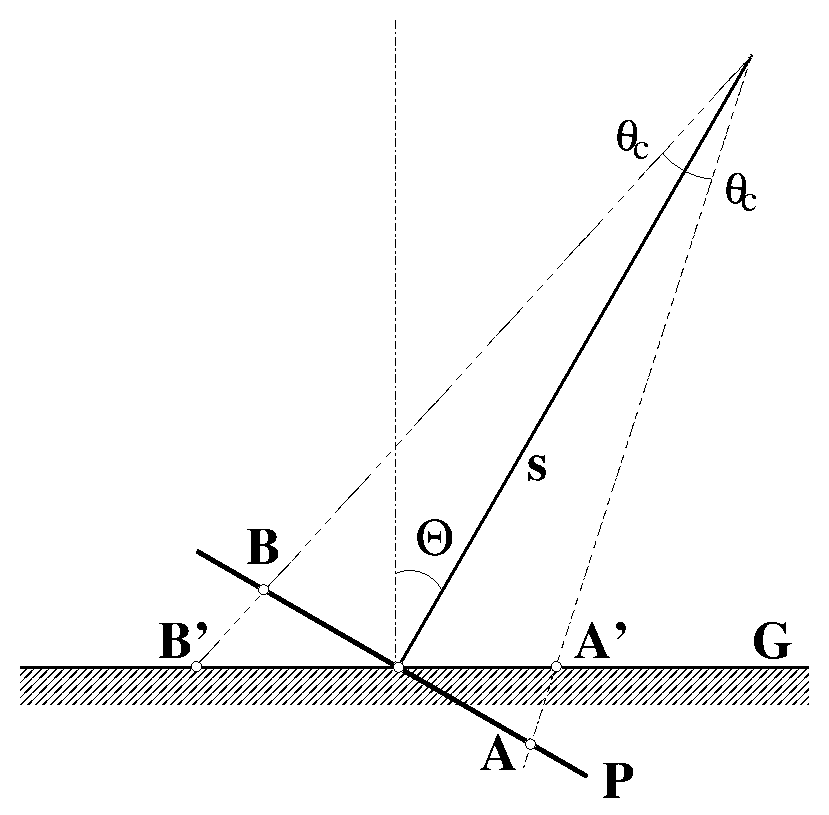
\includegraphics[width=.4\textwidth]{humpsketch}}
  \hfill\mbox{}
  \caption{(a) Sketch of the focussing of the \Cherenkov light in 
    the atmosphere. (b) Geometrical construction used in our
    \emph{toy-model}.}
  \label{fig:humpfigs}
\end{figure}

\begin{figure}[tb]
  \centering 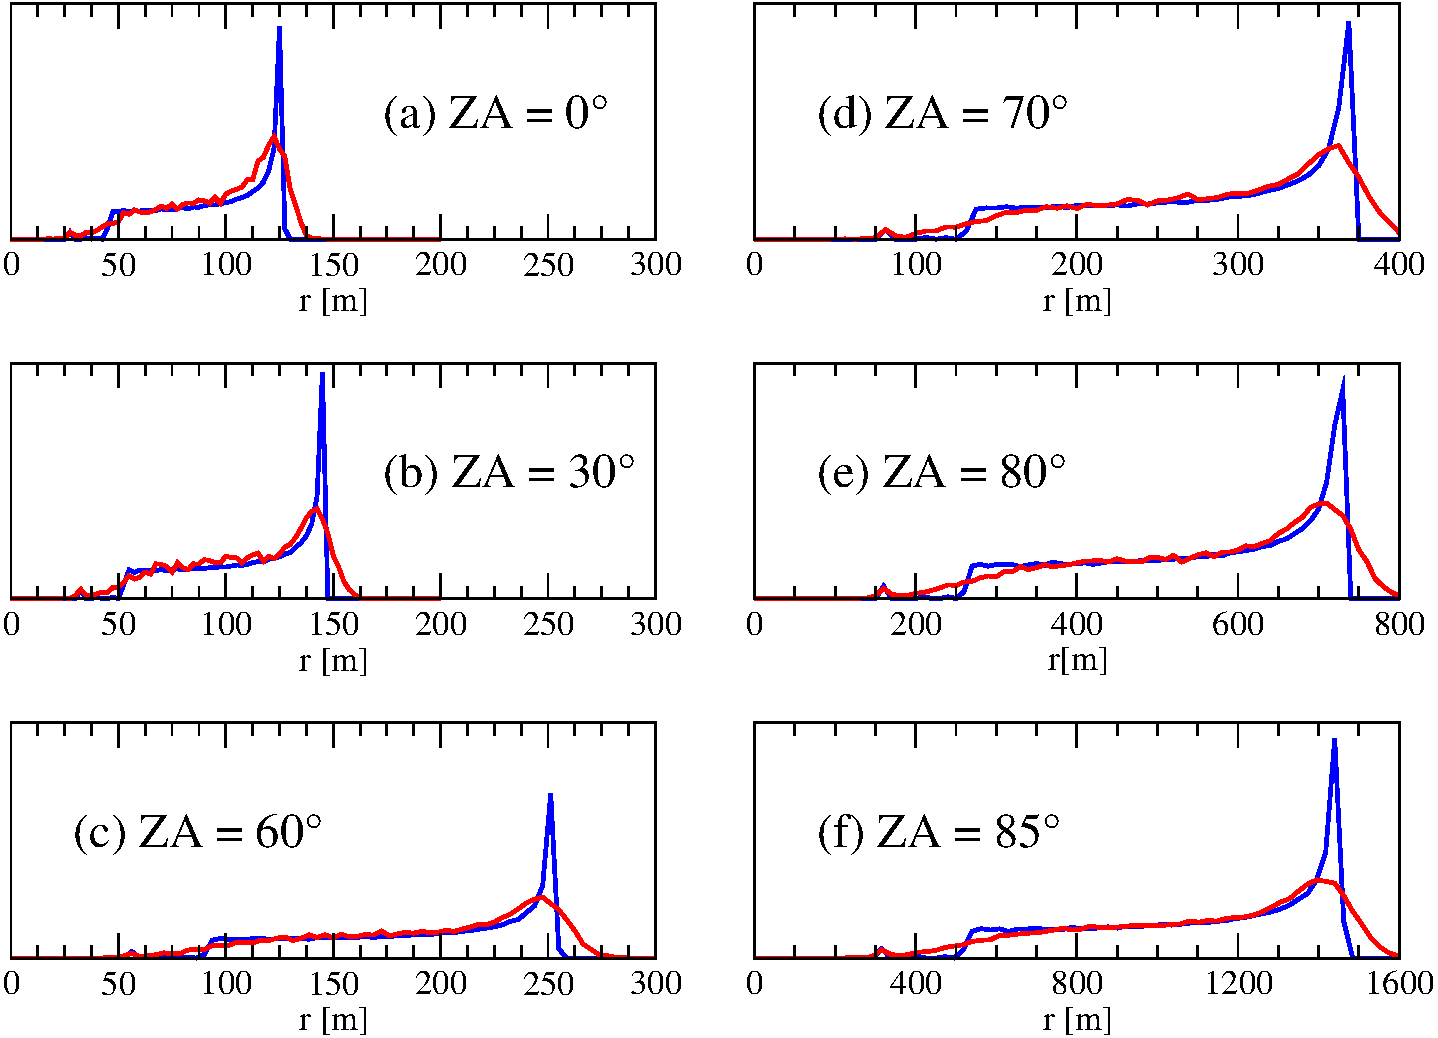
\includegraphics[width=.90\textwidth]{hump_ldist}
  \caption{Histograms of the hits of the \Cherenkov
    photons in the plane perpendicular to the trajectory of the
    charged particle, for different values of the Zenith Angle, in
    arbitrary units --- in blue, without smoothing; in red, with a
    gaussian smoothing function, assuming $\sigma(\theta_{\text{c}}) =
    0.05\text{\%}$. Note that in the first three histograms, (a)-(c),
    the scale in the X axis is the same, while in the last three,
    (d)-(f), the scale is doubling.}
  \label{fig:humpldist}
\end{figure}

\begin{figure}[tb]
  \centering 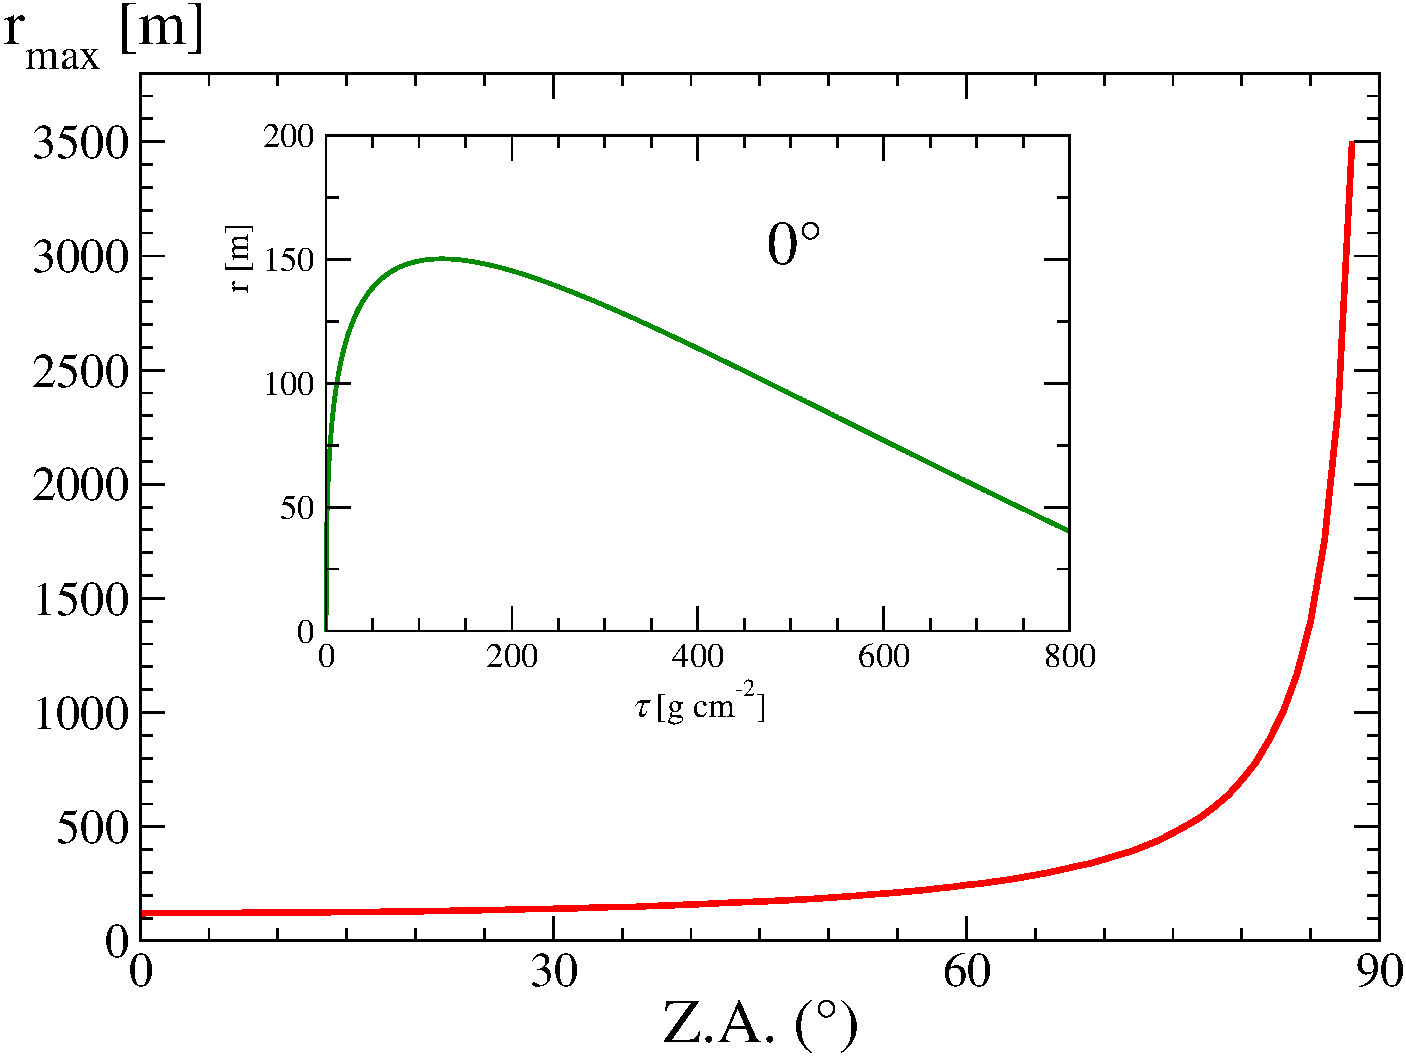
\includegraphics[width=.7\textwidth]{humps}
  \caption{Maxima of the radial distributions of \Cherenkov photons 
    obtained for different initial Zenith Angles. In the embeded
    graph, the theoretical values of the radial distances of the
    emitted \Cherenkov photons are shown as a function of the
    atmospheric thickness $\tau$, for Zenith Angle 0\deg. We can see that
    the theoretical value of the maximum $r$, around $150\u{m}$, is
    very close (and higher) to our calculated value of the position of
    the hump for 0\deg, $r_{\text{max}}\simeq125\u{m}$, as expected.}
  \label{fig:humps}
\end{figure}


%\begin{description}

%\item[\textbf{Rayleigh scattering}] The molecules in the atmosphere
%  produced scattering of the photons. This effects is strongly
%  correlated with the wavelength $\lambda$ of the light, being more
%  important for small wavelengths. The transmission coefficient due to
%  Rayleigh scattering is
%                                %
%  \Rayleigheq
%                                %
%  where $\tau_i = \tau_0 \exp(-h_i/H_{\mathrm{S}}) \sec\theta$ is the
%  \emph{slanted thickness} above a height $h_i$,
%  $\tau_{\mathrm{R}}(\lambda=400\u{nm}) = 2970\u{g/cm^2}$ is the mean
%  free path of the Rayleigh scattering in terms of thickness, $\tau_0
%  = 0.00129\u{g/cm^2}$, and $H_{\mathrm{S}} \simeq 7.5\u{km}$ is the
%  mentioned scale-height of the atmosphere.
  
%\item[\textbf{Mie scattering}] This effect is almost constant over the
%  whole range of optical wavelengths. It is due to the aerosol (dust)
%  particles suspended in the air, being its effect bigger at lower
%  heights. It depends also on the size of these particles. The
%  transmission coefficient is
%                                %
%  \Mieeq
%                                %
%  where $l_{\mathrm{M}}(400\u{nm}) \simeq 14\u{km}$ is the mean free
%  path for the Mie scattering, and $h_{\mathrm{M}} \simeq 1.2\u{km}$ is
%  the scale-height for the aerosol distribution.
  
%\item[\textbf{Ozone absorption}] This effect is very important in the
%  range 280--340\u{nm} and for low energy showers, in which most of
%  the \Cherenkov light emission is located where the density of ozone
%  is high.

%\end{description}

\endinput
%
%% Local Variables:
%% mode:latex
%% TeX-master: t
%% End:
%%EOF
